% ===========================================================================
%  02 — 背景与相关工作
%
%  事实来源：paper_context/paper_outline.md §2.2, §2.3
%  术语来源：paper_context/terminology.md
%  声明：     C-VLM-01, C-VLM-02, C-VLM-07（视觉事实本体）
% ===========================================================================
\chapter{背景与相关工作}\label{ch:background}

前一章将论文围绕一个需求展开：生成的程序化帮助应立足于可被检查的证据，并且这些
证据在学习者收到帮助前后均可被审查。本章解释该需求为何在 F/A-18C
冷启动任务中产生，以及它与现有工作的关系。第一部分介绍任务本身、可用的证据通道，
以及将座舱截图转化为结构化观察的视觉事实本体。第二部分将本论文置于智能教学系统、
基于模拟器的训练、基于规则的状态追踪、VLM
适配以及 AR/VR 中基于证据的辅助等研究领域的交叉点上。

% ===========================================================================
%  第一部分 — 领域背景
% ===========================================================================

% ---------------------------------------------------------------------------
\section{F/A-18C 冷启动任务}\label{sec:bg-coldstart}

% 证据：packs/fa18c_startup/pack.yaml
% 证据：packs/fa18c_startup/step_registry.yaml
% 证据：Doc/Evaluation/fa18c_startup_master.md

本论文研究的程序化场景为 DCS World 中的 F/A-18C
冷启动——一项将飞机从冷舱、不通电状态推至滑行就绪状态的前置座舱程序
~\citep{dcsworld,eagledynamics2023hornetguide}。该任务适合作为研究案例，因为它既
有界又对状态敏感。它有一组已知操作顺序，但成功完成取决于一些无法简化为文本检查单
的中间状态：在启动发动机之前必须先建立电源；在启动第二台发动机之前，发动机参数必
须进入标称范围；座舱显示器必须显示预期的页面；某些检查只有在较早的系统转换完成之
后才具有意义。

因此，对教学系统而言，冷启动的相关属性并不只是其步骤长度，而在于该程序迫使教学系
统综合三类证据：关于哪些步骤已完成的序列证据、关于座舱控制器和仪表状态的遥测证据，
以及关于显示页面内容的视觉证据。一个忽视其中任意一类信号的响应可能在局部表达流
畅，但在程序层面是错误的。

\subsection{程序结构：S01--S33 及阶段 P1--P6}

当前程序包将冷启动表示为 33 个编号步骤（S01--S33），分为六个阶段。本论文使用该
阶段结构来简洁描述任务对证据提出的需求：

\begin{description}
  \item[P1 (S01--S03)：] 上电与安全检查。电池及发电机启动、火警探测测试和 APU 启
    动为后续程序奠定了最初的电气与安全前置条件。
  \item[P2 (S04--S07)：] 右发动机启动。右发动机盘车、油门推进、引气循环以及
    注意/警告/提示灯测试引入了依赖遥测的时序与验证。
  \item[P3 (S08--S09)：] 显示器与通信。DDI、AMPCD、HUD、显示页面以及 COMM1 预置配
    置使显示状态成为程序证据链的一部分。
  \item[P4 (S10--S14)：] 左发动机与核心系统。左发动机启动、INS 对准模式选择、雷
    达开机和 OBOGS 激活均依赖于较早的发动机和航电状态。
  \item[P5 (S15--S27)：] FCS 与飞控。FCS 复位与 BIT、襟翼/配平配置、弹射杆和拦
    阻钩检查、受油管检查以及空速管加温配置将遥测可观测的控制动作与基于显示的确认
    相结合。
  \item[P6 (S28--S33)：] 滑行前仪表与最终检查。停机刹车、BINGO 燃油、高度表调
    校、备用姿态指示仪开锁以及姿态源选择完成滑行就绪状态。
\end{description}

每个步骤在程序包中均以前置条件和完成门控来表示。这些门控明确规定了教学系统在将某
个步骤视为可用或完成之前，哪些前置步骤和哪些状态变量必须得到满足。例如，右发动机
盘车步骤依赖于 APU 的支持，而左发动机启动则依赖于右发动机参数（如转速、温度、燃
油流量、喷口位置和滑油压力）进入标称范围。正因如此，该任务是验证基于证据的帮助的
有效测试案例：一个仅凭检查单顺序推进学习者的教学系统可能会忽略实际的飞机状态。

\subsection{座舱显示器与复合面板}

% 证据：packs/fa18c_startup/vision_layout.yaml
% 证据：DCS/Scripts/Export.lua
% 证据：Doc/Vision/Reports/qwen35_vlm_finetune_report_EN.md §1

冷启动中的许多状态在 F/A-18C
的座舱显示器上可见，而非直接作为简单的遥测变量提供。因此，视觉管线操作于一个包含
三个显示区域的固定复合面板图像之上：

\begin{itemize}
  \item \textbf{左 DDI（数字显示指示器）：} 在程序中用于诸如 FCS、SUPT 和 TAC
    等页面。在评估的冷启动流程中，FCS 页面及 FCS 页面标记是重要的视觉确认。
  \item \textbf{AMPCD（先进多用途彩色显示器）：} 用于 HSI 页面、地图图层和 INS
    对准文本。这些状态对与对准相关的视觉事实至关重要。
  \item \textbf{右 DDI：} 用于 BIT 根页面和 FCS-MC BIT 序列，包括中间状态、测试
    进行中和最终 GO 状态。
\end{itemize}

使用复合图像使训练与推理保持一致：模型在数据集构建、基准测试和运行时采集过程中看
到的是相同的三显示器布局。更重要的是，复合面板定义了一个狭窄的感知边界。VLM
不需要解释整个 VR 场景，也不需要推断飞行员的意图，而只需报告特定的座舱显示事实在
已知区域中是否可见。

\subsection{DCS-BIOS 遥测}

% 证据：adapters/dcs_bios/receiver.py
% 证据：adapters/telemetry_pipeline.py
% 证据：packs/fa18c_startup/telemetry_map.yaml

DCS-BIOS 为运行时提供了主要的非视觉证据来源。它通过 UDP 遥测流从 DCS World
导出座舱开关位置、指示器、警告灯、仪表和其他仪器状态
\citep{dcsbiosdocs}。教学运行时将该流标准化为稳定的变量，如 \texttt{rpm\_r}、
\texttt{apu\_ready} 和 \texttt{ins\_mode}，并应用差值消抖以减少抖动，同时追踪某
个数据源是缺失而非仅仅为假。

在遥测可覆盖的范围内，该通道具有权威性。诸如电池电源、油门动作、雷达模式和许多最
终滑行前开关状态等步骤无需计算机视觉即可检查。然而，DCS-BIOS 并不导出冷启动教学
系统所需的所有显示页面内容。因此，运行时仅将视觉用于遥测无法观测的状态，例如
FCS 页面、BIT 根页面、FCS-MC BIT 结果或 INS 对准文本是否可见。
图~\ref{fig:bg-evidence-sources} 总结了这一证据分工在 33 个步骤中的分布。

\begin{figure}[htbp]
  \centering
  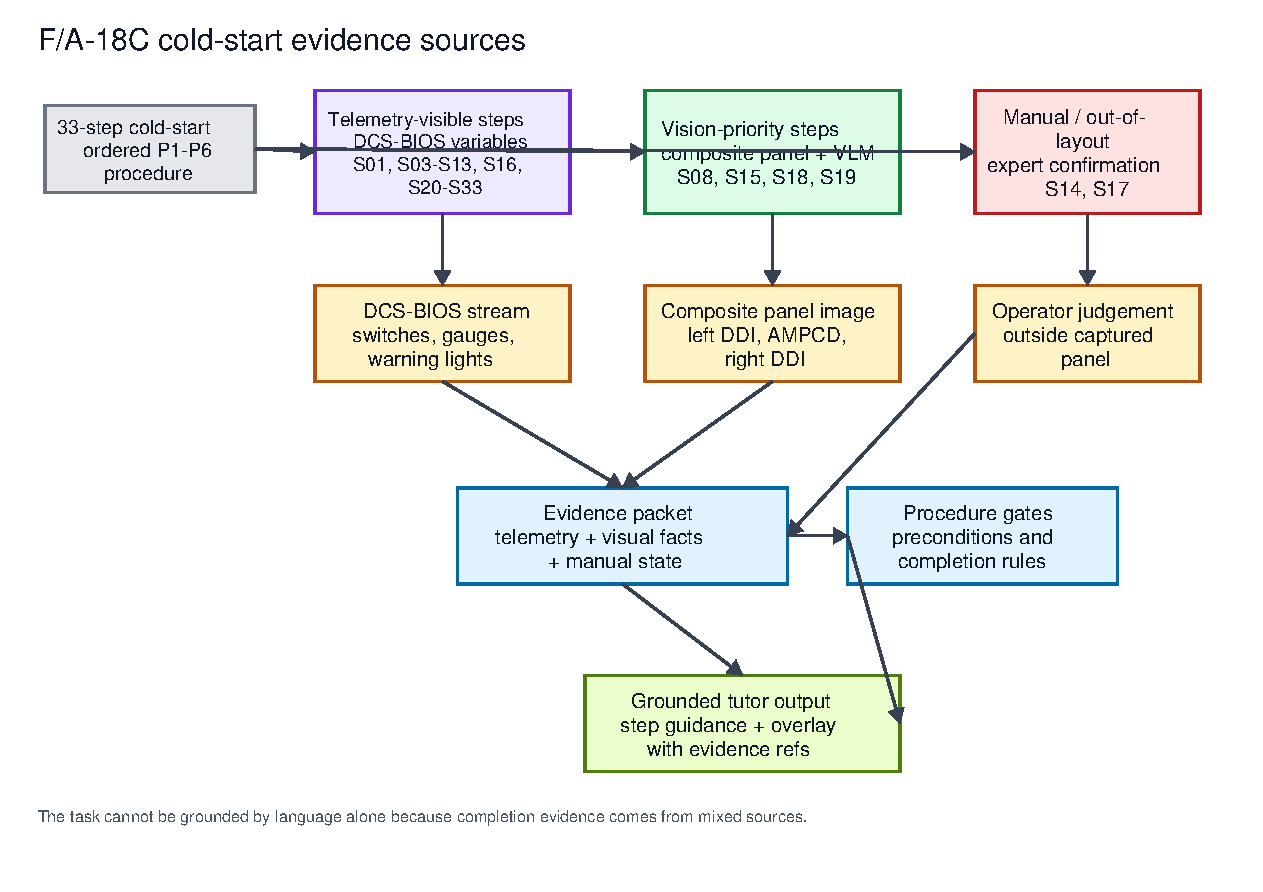
\includegraphics[width=\textwidth]{figures/fig_bg_evidence_sources.pdf}
  \caption{F/A-18C 冷启动任务的证据来源。33
  步骤程序结合了遥测可见步骤、视觉优先的显示检查以及少量手动或超出布局范围的确认；
  下游教学决策立足于相应证据来源，而非仅仅依赖语言模型的输出。}
  \label{fig:bg-evidence-sources}
\end{figure}

% ---------------------------------------------------------------------------
\section{视觉事实本体}\label{sec:bg-facts}

% 证据：packs/fa18c_startup/vision_facts.yaml
% 证据：core/vision_facts.py
% 证据：Doc/Vision/Reports/qwen35_vlm_finetune_report_EN.md §1
% 声明：C-VLM-01, C-VLM-02, C-VLM-07

视觉事实本体是感知与程序推理之间的契约。运行时并非要求 VLM
直接输出诸如"学习者下一步应按此按钮"之类的教学决策，而是要求其产生一小
组关于可见座舱显示状态的结构化命题。每个事实是一个离散观察，具有以下三种取值之一：

\begin{description}
  \item[\texttt{seen}：] 指定的视觉证据清晰存在；
  \item[\texttt{not\_seen}：] 指定的视觉证据不存在或不可辨识；
  \item[\texttt{uncertain}：] 图像质量、遮挡、裁剪或显示状态不足以做出有信心的判断。
\end{description}

这一表示方式有意避免了将感知与任务解释混为一谈。VLM 报告视觉证据是否可见，程序引
擎随后将这些事实与遥测数据、序列状态和步骤绑定结合起来，以判断某个步骤是已确认、
待定还是被阻止。因此，该本体并非一个次要的实现细节；它界定了模型被允许做出的断言
类型。

\subsection{从 8 事实 v1 到 13 事实 v2}

% 证据：datasets/vision_sft/stats.json（8 事实 v1）
% 证据：packs/fa18c_startup/vision_facts.yaml（13 事实 v2）
% 证据：Doc/Vision/Reports/qwen35_vlm_finetune_report_EN.md §8

该本体经历了两代演进。第一版包含覆盖左 DDI、右 DDI 和 AMPCD 的八个事实。它包括
了有用的显示级目标，如 FCS 页面可见性、BIT 页面可见性、FCS-MC 页面状态和 INS
对准页面可见性，同时也包含了诸如 \texttt{ins\_go}
这样的复合目标，要求模型从单一视觉帧中推断出一个高层的程序完成状态。

这一设计产出了一个清晰的教训。基于 180 张人工审核过的 Run-001 图像训练的第一个
LoRA 适配器虽然在分布内行为有所改善，但在独立的 Run-002 保留集上产生了严重的误
判：在 50 个样本中有 13 个样本被预测为 \texttt{ins\_go} 的 \texttt{seen}，而人工标
签为 \texttt{not\_seen}。这一错误不仅是模型的失败，更暴露了目标本身的设计问题：
\texttt{ins\_go} 将视觉感知与程序解释混为一谈。

第二代本体用 13 个可观察的视觉原子替代了此类复合目标：

\begin{center}
\footnotesize
\begin{tabular}{@{}ll@{}}
\textbf{区域} & \textbf{视觉事实} \\
\hline
左 DDI & \texttt{tac\_page\_visible} \\
左 DDI & \texttt{supt\_page\_visible} \\
左 DDI & \texttt{fcs\_page\_visible} \\
左 DDI & \texttt{fcs\_page\_x\_marks\_visible} \\
右 DDI & \texttt{bit\_root\_page\_visible} \\
右 DDI & \texttt{fcsmc\_page\_visible} \\
右 DDI & \texttt{fcsmc\_intermediate\_result\_visible} \\
右 DDI & \texttt{fcsmc\_in\_test\_visible} \\
右 DDI & \texttt{fcsmc\_final\_go\_result\_visible} \\
AMPCD & \texttt{hsi\_page\_visible} \\
AMPCD & \texttt{hsi\_map\_layer\_visible} \\
AMPCD & \texttt{ins\_grnd\_alignment\_text\_visible} \\
AMPCD & \texttt{ins\_ok\_text\_visible} \\
\end{tabular}
\end{center}

重要的变化不只是标签数量的增加，而在于本体从程序级判断转向了可观察的证据。例如，
v1 的 \texttt{ins\_go} 目标被分解为上表中所示的 AMPCD
文本和地图图层观察，程序引擎随后决定这些观察如何与对准步骤关联。这一设计原则承载
了论文 VLM 部分的主要科学洞察：VLM 应提取局部视觉证据，而程序含义应由显式的下游
规则来赋予。

\subsection{粘性事实与步骤绑定}

% 证据：packs/fa18c_startup/vision_facts.yaml（sticky、step_bindings）
% 证据：core/vision_facts.py（merge_vision_fact_observation、facts_satisfy_step_binding）

两种运行时机制使本体在实时帮助周期中可用。

\paragraph{粘性事实。}
某些视觉事件是瞬态的，但在程序上具有重要意义。例如，
\texttt{fcsmc\_final\_go\_result\_visible} 事实被标记为粘性，有效期为 600
秒。一旦它被观察为 \texttt{seen}，后续帧中出现的 \texttt{not\_seen} 或
\texttt{uncertain} 不会立即清除该证据。这防止了已完成的视觉事件仅仅因为学习者切换
了页面、显示器闪烁或采集窗口错过了相关时刻而消失。非粘性事实（如页面可见性事实）
则快速过期并被持续重新评估。

\paragraph{步骤绑定。}
视觉事实仅通过 \texttt{vision\_facts.yaml}
中的显式绑定才具有程序意义。绑定指定了某个步骤要被视觉确认所必须可见的事实。某些
绑定要求所有列出的事实同时满足，例如 S08 同时要求左 DDI 上的 FCS 页面和右 DDI 上
的 BIT 根页面。其他绑定则在多个视觉线索可以支撑同一程序状态时允许选择其一。

程序包还根据每个步骤的首选证据来源对其进行分类：

\begin{itemize}
  \item \texttt{bios\_priority\_steps} 用于遥测可见的状态；
  \item \texttt{vision\_priority\_steps} 用于依赖显示的状态；
  \item \texttt{manual\_or\_out\_of\_layout\_steps} 用于需要人工确认或超出三显示器
    复合面板范围的状态。
\end{itemize}

这一分类是论文基于证据原则的实际表达：每个步骤在被用于教学之前，都要经过最可靠可
用信号的校验。

% ===========================================================================
%  第二部分 — 相关工作
% ===========================================================================

% ---------------------------------------------------------------------------
\section{智能教学系统与程序化训练}\label{sec:rw-tutoring}

智能教学系统（ITS）为本工作提供了最接近的教育范式先例。经典的 ITS 研究区分专家知
识、学习者状态和教学反馈，并已证明基于步骤的计算机教学系统在结构化学习领域中具有
效性~\citep{vanlehn2011relative}。在程序化情境中，基于约束和示例追踪的
教学系统对期望行为进行建模，并将学习者行为与作者编写的任务知识进行比对
\citep{mitrovic2012constraint,aleven2009example}。这些思想直接启发了本论文
中程序包和门控规则的使用。

区别在于观察接口。许多 ITS 运行在学习者行为已表示为形式化事件的环境之中，而本工作
所用的模拟器并非面向教学系统原生设计。运行时必须从 DCS-BIOS
遥测、截图、序列历史和偶发的人工确认中推断程序状态，这使得证据整合本身成为教学问
题的一部分。

LLM 带来了进一步的张力。它们能够产生流畅且灵活的教学对话，近期的教育讨论既认识到
其潜力，也认识到其可靠性风险~\citep{kasneci2023chatgpt}。对于座舱程序而言，
仅凭流畅是不够的。因此，本论文的贡献并非一个开放式的 LLM
教学系统，而是一个受约束的教学运行时：其中生成的语言位于证据采集、检索、程序推理
和验证的下游。

% ---------------------------------------------------------------------------
\section{基于模拟器的训练与仪表化}\label{sec:rw-sim}

基于模拟器的航空训练是一个成熟的领域，已有研究考察了模拟如何支持飞行训练情境中的
技能习得与迁移~\citep{hays1992flight}。DCS World 提供了本论文所使用的高保真
仿真环境~\citep{dcsworld}。对本工作而言，相关的研究问题是仪表化：教学系
统如何在不用自定义教学接口替换模拟器的前提下，观测学习者和飞机正在做什么。

DCS-BIOS 通过一个结构化的遥测桥接暴露座舱状态，部分解决了这一问题
~\citep{dcsbiosdocs}。与单纯的屏幕采集相比，遥测提供了对许多开关位置、指示器
状态和数值的确定性访问。然而，遥测并不覆盖冷启动所需的每一条证据，尤其是显示页面
内容和文本。因此，本论文将模拟器仪表化视为一个多模态问题：在遥测可靠且直接的地方
使用遥测，而视觉则保留用于遥测不导出的座舱证据。

这种分工也改善了可审计性。一个记录下来的帮助周期事后可以展示哪些状态来自
DCS-BIOS、哪些事实来自 VLM、哪条规则使某个步骤具备资格或处于阻塞状态，以及哪些检
索到的来源支撑了所生成的解释。仪表化因此不仅是一个工程需求，更是评估教学系统行为
的前提条件。

% ---------------------------------------------------------------------------
\section{基于规则与状态感知的教学}\label{sec:rw-state}

教学运行时将确定性状态追踪与模型生成的语言相结合。基于规则的程序追踪方法——包括有
限状态机、产生式规则和面向约束的模型——因其显式地呈现任务结构而具有可解释性。本论
文的程序包遵循这一原则：步骤、前置条件、完成门控、视觉绑定和错误分类均以声明式配
置形式编写，而非隐藏在提示词中。

纯规则式教学系统的局限性在于，当学习者在意外状态下请求帮助或需要解释而非二元纠错
时，预编写的反馈可能变得脆弱。因此，运行时将自然语言的构造委托给 LLM，但不将决定
程序状态的权力交给它。步骤推理、资格判定、证据可用性和覆盖层白名单均保持在确定性
控制之下。

这种混合分工与将语言模型基于行动可行性和符号结构的更广泛研究相关，例如将语言基于
机器人能力的 SayCan 式
工~\citep{ahn2022saycan}。本论文将这种基于直觉扩展到模拟器教学中：在一
个生成的响应得以执行之前，必须将其与运行时能够观察、验证和回放的证据绑定在一起。

% ---------------------------------------------------------------------------
\section{基础模型与 VLM 用于情境化辅助}\label{sec:rw-vlm}

基础模型提供了两种对情境化教学有吸引力的能力：语言模型可以生成灵活的解释，视觉语
言模型可以从座舱图像中提取信息。参数高效微调方法，特别是低秩适配（LoRA），使得用
有限的课训练参数将大型模型适配到狭窄任务上成为可能
\citep{hu2021lora,mangrulkar2022peft}。本论文使用的模型骨干网络和 VLM
文献为这一适配环境提供了一般技术背景
~\citep{bai2023qwen,liu2023llava,dai2023instructblip}。

本论文以受限的方式使用这些能力。VLM 不负责生成自由形式的座舱描述，LLM
也不负责凭空推断下一个程序状态。相反，VLM
输出结构化的 JSON 视觉事实，帮助生成模型接收由运行时组装好的证据包。这一选择遵循
了与检索增强生成相同的一般动机：模型输出应以显式外部证据为条件，而非仅依赖参数化
记忆~\citep{lewis2020rag}。

座舱显示任务也与结构化屏幕理解类似。针对 GUI
和屏幕内容理解的研究表明，视觉模型可以对固定区域、标签和符号化布局进行推理
\citep{wang2021screen2words}。座舱显示器具有相同的结构化特征，但教学环
境对误报施加了更严格的后果：一个 VLM 如果错误地将关键显示状态报告为可见，可能导
致教学系统在错误的时间推进学习者。正因如此，本体设计和关键误报分析在本论文中被视
为核心方法论问题，而非次要的基准细节。

% ---------------------------------------------------------------------------
\section{AR/VR 中的可解释与基于证据的 AI 辅助}\label{sec:rw-xai}

初始提案曾将教学系统部署于沉浸式 Quest~3 座舱体验中，所实现的系统通过 VR
先导研究保留了这一评估方向。先前关于面向维护和程序化任务的 AR
指导的研究展现了在用户任务情境中呈现指令的价值，通常通过空间注册的文本、箭头或动
画来实现~\citep{palmarini2018ar}。这类系统说明了情境内指导为何有吸引
力：学习者可以将注意力保持在任务环境上，而无需切换到外部材料。

本文研究的系统不同于预编写的 AR 指导，因为它生成的帮助内容是在运行时根据当前证据
动态产生的，这使得可解释性和可追溯性成为核心议题。关于可解释 AI 和人机交互的工
作强调，用户和开发者需要理解系统为何产生了某个推荐，尤其是在高风险或安全敏感的场
景下~\citep{gunning2019xai,amershi2019guidelines}。在本论文中，解释需求
通过证据引用得以具体落实：每个被推荐的步骤、覆盖层目标或拒绝推进的决定
都可以追溯至遥测、某条规则、某个视觉事实或某条检索到的来源。

这种基于证据的要求也限制了关于 VR 的声明。第~\ref{ch:evaluation} 章中的先导研究
表明，运行时和仪表化可以在 VR 中由真实参与者验证运行，但该研究并未建立受控的教育
效果。因此，VR 的贡献属于评估框架和形成性证据的一部分，而论文的主要声明仍然是基
于证据的教学运行时的设计与验证。

% ---------------------------------------------------------------------------
\section{本工作的定位}\label{sec:rw-positioning}

本论文位于上述各个领域的交叉点上，但其贡献在于特定的集成方式，而非单纯归属于任
何单一领域。从智能教学系统中，它汲取了对显式任务模型和状态敏感反馈的需求。从模拟
器训练中，它汲取了在高保真环境中观测真实学习者行为所需的仪表化能力。从基于规则的
辅助中，它汲取了确定性程序门控。从基础模型工作中，它汲取了灵活的语言生成和领域适
配的视觉提取能力。从可解释性及 AR/VR 辅助中，它汲取了帮助在情境中保持可审查性的
要求。

所得到的系统是一个基于证据的程序化教学运行时。其程序包定义了什么算作有效的状态证
据；DCS-BIOS 在可用处提供遥测；视觉事实本体在遥测缺失处提供结构化的座舱显示观
察；检索提供程序化源材料；帮助周期通过验证、白名单、回退、日志记录和回放来约束模
型输出。这是本论文后续章节中发展的研究立场。

声明边界同样重要。技术章节和基准测试评估了该架构和视觉事实管线是否能够为教学产生
可靠、可审计的证据。形成性 VR
先导研究提供了关于可行性、任务完成情况、错误模式和仪表化在真实参与者中的描述性证
据。在能够对学习收益、工作负荷降低、记忆保持或技能迁移做出声明之前，仍需要更大规
模的受控研究。
